\subsection{Execution Model}

The \definition{CUDA execution model} \textbf{defines how parallel computing tasks are organized and executed on NVIDIA GPUs}. It consists of both software and hardware components that work together to efficiently process large amounts of data in parallel.

\begin{flushleft}
    \textcolor{Green3}{\faIcon{tools} \textbf{Software Hierarchy}}
\end{flushleft}
\begin{itemize}
    \item \important{Grid}. A grid is a \textbf{collection of thread blocks that execute a given kernel function}. Each grid is associated with a specific kernel launch. Grids can be one-dimensional, two-dimensional, or three-dimensional, depending on the problem's complexity.

    \item \important{Thread Block}. A thread block is a \textbf{group of threads that execute together and can cooperate by sharing data through shared memory}. Each block is \underline{independent}, allowing the scheduler to execute blocks in any order. Thread blocks can also be organized in one, two, or three dimensions.

    \item \important{Thread}. The \textbf{smallest unit of execution in CUDA}. Each thread executes the \textbf{same code but operates on different data elements}. Threads within a block can communicate and synchronize with each other, enabling collaborative computation.
\end{itemize}

\begin{flushleft}
    \textcolor{Green3}{\faIcon{memory} \textbf{Hardware Hierarchy}}
\end{flushleft}
\begin{itemize}
    \item \important{GPU}. The \textbf{physical hardware that executes the parallel tasks}. A GPU consists of \textbf{multiple Streaming Multiprocessors (SMs)}.

    \item \important{Streaming Multiprocessor (SM)}. Each SM can \textbf{execute multiple threads concurrently}. Thread blocks are assigned to SMs for execution. SMs manage and execute warps of threads.

    \item \important{GPU Core}. \textbf{Individual cores within the SMs that perform the actual computation}. Cores \textbf{execute threads in groups called warps}, typically comprising 32 threads.
\end{itemize}
\begin{figure}[!htp]
    \centering
    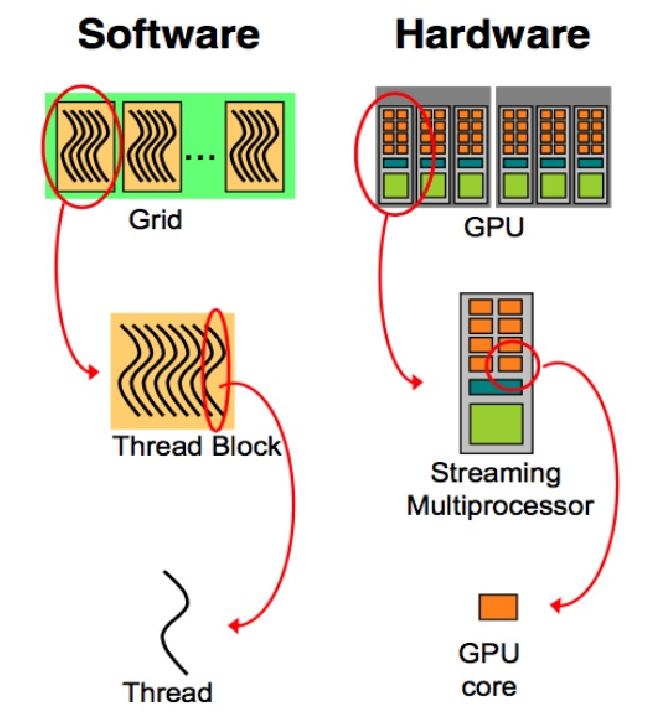
\includegraphics[width=.5\textwidth]{img/cuda-execution-model-1.pdf}
    \caption{Graphical representation of the CUDA execution model.}
\end{figure}

\highspace
\begin{flushleft}
    \textcolor{Red2}{\faIcon{exclamation-triangle} \textbf{What happens if the kernel startup doesn't match the input dataset?}}
\end{flushleft}
\textbf{Execution configuration mismatches occur when the number of\break threads configured for a kernel launch does not perfectly match the size of the dataset being processed}. This can lead to \emph{inefficiencies} or the need for \emph{additional handling in the kernel code}.
\begin{itemize}
    \item \important{Optimal Thread Configuration}: \textbf{multiple of 32 threads}. It's generally desirable to configure blocks with a multiple of 32 threads for performance reasons. This is because GPUs execute threads in groups of 32, known as warps. Ensuring the number of threads per block is a multiple of 32 can prevent under-utilization of GPU resources.

    As the warp dimension changes, the optimal thread configuration should also change.

    \item \important{Dealing with Non-Multiple of 32 threads}. If the dataset size (e.g., \texttt{N=1000}) is not a multiple of 32, we can create more than 1000 threads and use an extra check within the kernel to handle the excess threads.
    \begin{enumerate}
        \item We pass the dataset size \texttt{N} as an argument to the kernel.
        \item Inside the kernel, we check if the thread ID is greater than or equal to \texttt{N}. If it is, those threads should not perform any operations.
        \begin{lstlisting}[language=C++]
__global__ void kernelFunction(float* data, int N) {
    int tid = blockIdx.x * blockDim.x + threadIdx.x;
    if (tid < N) {
        // Perform operations only if thread ID
        // is within the dataset size
        data[tid] = data[tid] * 2.0f;
    }
}
        \end{lstlisting}
    \end{enumerate}

    \item \important{Insufficient threads}. In some cases, there may be fewer threads than data elements to process, either for performance reasons or because the dataset is very large.

    In this case, the solution is using a \textbf{Stride Factor}. We can use a stride factor \textbf{corresponding to the total number of threads}. The stride factor is calculated as \texttt{gridDim.x * blockDim.x}, representing the \textbf{total number of threads in the grid}. Each thread processes multiple elements by iterating with a step size equal to the stride.
    \begin{lstlisting}[language=C++]
__global__ void kernelFunctionWithStride(float* data, int N) {
    int tid = blockIdx.x * blockDim.x + threadIdx.x;
    int stride = gridDim.x * blockDim.x;
    for (int i = tid; i < N; i += stride) {
        data[i] = data[i] * 2.0f;
    }
}
    \end{lstlisting}
\end{itemize}